\section{Sở GD \& ĐT Hà Nội NĂM HỌC 25--26, Lần 1}
\caulc
\Opensolutionfile{ans}[ans/ans-26-6-HaNoi-SoGD-L1-LC]
\begin{ex}%[Đề thi thử Sở GD Hà Nội 2025-2026 L1]%[Thái Doãn Hùng, dự án đề THPT 2025 2026]%[1D1H4-2]
	Tập xác định của hàm số $y=\tan x$ là
	\choice
	{\True $\mathbb{R}\setminus\left\{\dfrac{\pi}{2}+k\pi \ \mid\ k\in\mathbb{Z}\right\}$}
	{$\mathbb{R}\setminus\left\{\dfrac{\pi}{2}+k2\pi \ \mid\ k\in\mathbb{Z}\right\}$}
	{$\mathbb{R}\setminus\left\{k\pi \ \mid\ k\in\mathbb{Z}\right\}$}
	{$\mathbb{R}\setminus\left\{k2\pi \ \mid\ k\in\mathbb{Z}\right\}$}
	\loigiai
	{
	Hàm số $y=\tan x$ xác định khi và chỉ khi $\cos x \ne 0 \Leftrightarrow x \ne \dfrac{\pi}{2}+k\pi,\ k\in\mathbb{Z}$.\\
	Vậy tập xác định của hàm số là $\mathscr{D}=\mathbb{R}\setminus\left\{\dfrac{\pi}{2}+k\pi \ \middle|\ k\in\mathbb{Z}\right\}$.
	}
\end{ex}
		
\begin{ex}%[Đề thi thử Sở GD Hà Nội 2025-2026 L1]%[Thái Doãn Hùng, dự án đề THPT 2025 2026]%[1D2N3-4]
	Cho cấp số nhân $(u_n)$ có số hạng đầu tiên $u_1=3$ và công bội $q=-2$. 
	Số hạng thứ tư của cấp số nhân đã cho là
	\choice
	{\True $u_4=-24$}
	{$u_4=48$}
	{$u_4=-4$}
	{$u_4=-48$}
	\loigiai
	{
	Ta có $	u_n=u_1\cdot q^{n-1} (n\in \mathbb{N}^*,n>1)$.\\
	Suy ra $u_4=3\cdot(-2)^3=-24$.
	}
\end{ex}
	
\begin{ex}%[Đề thi thử Sở GD Hà Nội 2025-2026 L1]%[Thái Doãn Hùng, dự án đề THPT 2025 2026]%[2H2N2-3]
	Trong không gian với hệ trục tọa độ $Oxyz$, cho vectơ $\vec{u}=3\vec{i}-2\vec{j}+\vec{k}$. Tọa độ của vectơ $\vec{u}$ là
	\choice
	{$(1;3;-2)$}
	{$(-2;3;1)$}
	{$(3;1;-2)$}
	{\True $(3;-2;1)$}
	\loigiai
	{
	Ta có $\vec{u}=3\vec{i}-2\vec{j}+\vec{k} $ nên tọa độ của vectơ $\vec{u}$ là $(3;-2;1)$.
	}
\end{ex}
		
\begin{ex}%[Đề thi thử Sở GD Hà Nội 2025-2026 L1]%[Thái Doãn Hùng, dự án đề THPT 2025 2026]%[2D4N3-3]
	Cho hàm số $y=f(x)$ liên tục và không âm trên đoạn $[0;2]$. Thể tích khối tròn xoay sinh ra khi quay quanh trục $Ox$ hình phẳng giới hạn bởi đồ thị hàm số $y=f(x)$, trục hoành và hai đường thẳng $x=0$, $x=2$ là
	\choice
	{$\pi\displaystyle\int\limits_0^2 f(x)\mathrm{\,d}x$}
	{\True $\pi\displaystyle\int\limits_0^2 \left[f(x)\right]^2\mathrm{\,d}x$}
	{$\displaystyle\int\limits_0^2 f(x)\mathrm{\,d}x$}
	{$\displaystyle\int\limits_0^2 \left[f(x)\right]^2\mathrm{\,d}x$}
	\loigiai
	{
	Thể tích khối tròn xoay sinh ra khi quay hình phẳng quanh trục $Ox$ được tính theo công thức \[ V=\pi \displaystyle \int\limits_a^b \left[f(x)\right]^2\mathrm{\,d}x\].
	Với $a=0$, $b=2$ ta được $V=\pi \displaystyle \int\limits_0^2 \left[f(x)\right]^2\mathrm{\,d}x.	$
	}
\end{ex}

\begin{ex}%[Đề thi thử Sở GD Hà Nội 2025-2026 L1]%[Thái Doãn Hùng, dự án đề THPT 2025 2026]%[2H2H1-2]
	\immini{
	Cho hình hộp $ABCD.A'B'C'D'$ \textit{(tham khảo hình vẽ)}. Khi đó, tổng $\overrightarrow{AB}+\overrightarrow{AD}+\overrightarrow{DD'}$ bằng
	\choice
	{\True $\overrightarrow{AC'}$}
	{$\overrightarrow{C'A}$}
	{$\overrightarrow{D'A}$}
	{ $\overrightarrow{AD'}$}
	}
	{
	\begin{tikzpicture}[line join=round,line cap=round,>=stealth,scale=0.5]
		\coordinate (B) at (0,0);
		\coordinate (C) at (4,0);
		\coordinate (D) at (5,1.2);
		\coordinate (A) at ($(B)+(1,1.2)$);
		\coordinate (B') at ($(B)+(0.4,2.6)$);
		\coordinate (C') at ($(C)+(0.4,2.6)$);
		\coordinate (D') at ($(D)+(0.4,2.6)$);
		\coordinate (A') at ($(A)+(0.4,2.6)$);
		\draw (B) -- (C) (C) -- (D) (D) -- (D') (D') -- (C') (C') -- (B') (B') -- (B) (C') -- (C);
		\draw[dashed] (A) -- (B) (A) -- (D) (A) -- (A');
		\draw (A') -- (B') (A') -- (D');
		\foreach \p in {A,B,C,D,A',B',C',D'} \fill (\p) circle (1.5pt);
		\foreach \p in {A,B,B'} \node[left] at (\p) {$\p$};
		\foreach \p in {C,D,C',D'} \node[right] at (\p) {$\p$};
		\foreach \p in {A'} \node[above] at (\p) {$\p$};
	\end{tikzpicture}
	}
	\loigiai
	{
	Ta có $\overrightarrow{AB}+\overrightarrow{AD}=\overrightarrow{AC}$.\\
	Suy ra $\overrightarrow{AB}+\overrightarrow{AD}+\overrightarrow{DD'}
	=\overrightarrow{AC}+\overrightarrow{CC'}
	=\overrightarrow{AC'}$.
	}
\end{ex}

\begin{ex}%[Đề thi thử Sở GD Hà Nội 2025-2026 L1]%[Thái Doãn Hùng, dự án đề THPT 2025 2026]%[1H8H7-2]
	Cho hình chóp $O.ABC$ có $OA$, $OB$, $OC$ đôi một vuông góc với nhau và $OA=a$, $OB=b$, $OC=c$. Thể tích của khối chóp $O.ABC$ bằng
	\choice
	{$\dfrac{abc}{3}$}
	{\True $\dfrac{abc}{6}$}
	{$\dfrac{abc}{2}$}
	{$abc$}
	\loigiai
	{
	Vì $OA$, $OB$, $OC$ đôi một vuông góc nên thể tích của khối chóp được tính bởi công thức: \[V=\dfrac{1}{6}OA\cdot OB\cdot OC\].
	Suy ra $V=\dfrac{1}{6}\cdot a\cdot b\cdot c=\dfrac{abc}{6}$.
	}
\end{ex}

\begin{ex}%[Đề thi thử Sở GD Hà Nội 2025-2026 L1]%[Thái Doãn Hùng, dự án đề THPT 2025 2026]%[2D1H2-2]
	Cho hàm số $y=f(x)$ có đạo hàm trên $\mathbb{R}$ và có bảng xét dấu của $f'(x)$ như sau:
	\begin{center}
	
\begin{tikzpicture}
		\tkzTabInit[lgt=1.2,espcl=2] 
		{$x$/1,$f'(x)$/1}
		{$-\infty$,$-3$,$1$,$2$,$+\infty$}
		\tkzTabLine{,-,z,+,z,+,z,-,}
	\end{tikzpicture}
	\end{center}
	Số điểm cực trị của hàm số $y=f(x)$ là
	\choice
	{$0$}
	{$1$}
	{\True $2$}
	{$3$}
	\loigiai
	{
	Dựa vào bảng xét dấu của $f'(x)$, ta thấy $f'(x)$ đổi dấu qua $x=-3$ và $x=2$, không đổi dấu khi qua $x=1$. \\
	Nên hàm số có $2$ điểm cực trị.
	}
\end{ex}

\begin{ex}%[Đề thi thử Sở GD Hà Nội 2025-2026 L1]%[Thái Doãn Hùng, dự án đề THPT 2025 2026]%[1D5N1-4]
	Kết quả kiểm tra Toán của $40$ học sinh lớp $12A$ được cho bởi bảng sau:
	$$\begin{array}{|c|c|c|c|c|c|}
	\hline
	\textbf{Khoảng điểm} & [0;2) & [2;4) & [4;6) & [6;8) & [8;10] \\
	\hline
	\textbf{Số học sinh} & 0 & 8 & 15 & 10 & 7 \\
	\hline
	\end{array}$$
	Mốt của mẫu số liệu ghép nhóm trên thuộc khoảng điểm nào sau đây?
	\choice
	{$[6;8)$}
	{$[8;10]$}
	{$[2;4)$}
	{\True $[4;6)$}
	\loigiai
	{
	Mốt của mẫu số liệu ghép nhóm thuộc lớp có tần số lớn nhất.\\
	Ta thấy khoảng $[4;6)$ có tần số lớn nhất bằng $15$.\\
	Vậy mốt của mẫu số liệu ghép nhóm thuộc khoảng $[4;6)$.
	}
\end{ex}

\begin{ex}%[Đề thi thử Sở GD Hà Nội 2025-2026 L1]%[Thái Doãn Hùng, dự án đề THPT 2025 2026]%[2H5N1-2]
	Trong không gian với hệ trục tọa độ $Oxyz$, cho mặt phẳng $(P)\colon x-2y+2z-1=0$. Một vectơ pháp tuyến của mặt phẳng $(P)$ có tọa độ là
	\choice
	{$(-1;1;2)$}
	{\True $(1;-2;2)$}
	{$(1;2;2)$}
	{$(-1;-2;2)$}
	\loigiai
	{
	Mặt phẳng $(P)\colon x-2y+2z-1=0$ có một vectơ pháp tuyến là $\vec{n}=(1;-2;2)$.
	}
\end{ex}

\begin{ex}%[Đề thi thử Sở GD Hà Nội 2025-2026 L1]%[Thái Doãn Hùng, dự án đề THPT 2025 2026]%[2D4N1-2]
	Họ nguyên hàm của hàm số $f(x)=x^7$ là
	\choice
	{$\dfrac{x^7}{7}+C$}
	{$7x^6+C$}
	{$8x^8+C$}
	{\True $\dfrac{x^8}{8}+C$}
	\loigiai
	{
	Ta có $\displaystyle \int x^7\mathrm{\,d}x=\dfrac{x^8}{8}+C$.
	}
\end{ex}

\begin{ex}%[Đề thi thử Sở GD Hà Nội 2025-2026 L1]%[Thái Doãn Hùng, dự án đề THPT 2025 2026]%[1D6H4-3]
	Tập nghiệm của bất phương trình $\log_2(x-1)\le 3$ là
	\choice
	{$(-\infty;9]$}
	{$(1;9)$}
	{\True $(1;9]$}
	{$[1;9]$}
	\loigiai
	{
	Điều kiện xác định: $x-1>0 \Leftrightarrow x>1$.\\
	Vì cơ số $2>1$ nên	$ \log_2(x-1)\le 3 \Leftrightarrow x-1 \le 2^3\Leftrightarrow x \le 9$.\\
	Kết hợp điều kiện ta được $1<x\le 9$.\\
	Vậy tập nghiệm của bất phương trình là $(1;9]$.
	}
\end{ex}

\begin{ex}%[Đề thi thử Sở GD Hà Nội 2025-2026 L1]%[Thái Doãn Hùng, dự án đề THPT 2025 2026]%[2D1H3-2]
	\immini
	{Cho hàm số $y=f(x)$ có đồ thị như hình vẽ. Tổng của giá trị lớn nhất và giá trị nhỏ nhất của hàm số đã cho trên đoạn $[-2;2]$ bằng
	\choice
	{$-5$}
	{$0$}
	{$-1$}
	{\True $-6$}
	}
	{
	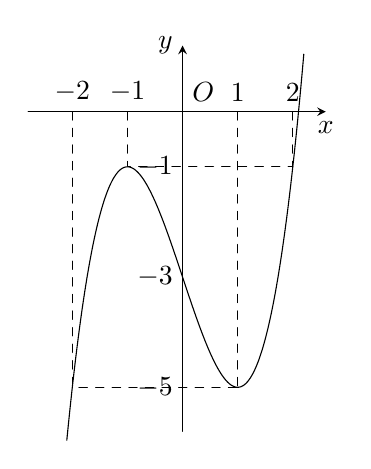
\begin{tikzpicture}[line join=round,line cap=round,>=stealth,scale=0.7]
		\draw[->] (-2.8,0)--(2.6,0) node[below] {$x$};
		\draw[->] (0,-5.8)--(0,1.2) node[left] {$y$};
		\draw[dashed] (-2,0)--(-2,-5)--(1,-5);
		\draw[dashed] (-1,0)--(-1,-1)--(2,-1);
		\draw[dashed] (1,0)--(1,-5);
		\draw[dashed] (2,0)--(2,-1);	
		\node[above right] at (0,0) {$O$};
		\node[above] at (-2,0) {$-2$};
		\node[above] at (-1,0) {$-1$};
		\node[above] at (1,0) {$1$};
		\node[above] at (2,0) {$2$};
		\node[left] at (0,-1) {$-1$};
		\node[left] at (0,-3) {$-3$};
		\node[left] at (0,-5) {$-5$};
		\draw[smooth,samples=200,domain=-2.1:2.2] plot(\x,{(\x)^3-3*(\x)-3});
	\end{tikzpicture}
	}
	\loigiai
	{
	Dựa vào đồ thị, trên đoạn $[-2;2]$ ta có $\max\limits_{x \in[-2;2]}f(x)=-1,\min\limits_{x \in[-2;2]}f(x)=-5$.\\
	Suy ra $\max\limits_{x \in[-2;2]}f(x)+\min\limits_{x \in[-2;2]}f(x)=-1+(-5)=-6$.
	}
\end{ex}
\Closesolutionfile{ans}

\cauds
\Opensolutionfile{ans}[ans/ans-26-6-HaNoi-SoGD-L1-DS]
\begin{ex}%[Đề thi thử Sở GD Hà Nội 2025-2026 L1]%[Thái Doãn Hùng, dự án đề THPT 2025 2026]%[2H5V1-5]
	\immini
	{Cho hình hộp chữ nhật $ABCD.A'B'C'D'$ có $AB=4$, $AD=3$ và $AA'=12$. Chọn hệ trục tọa độ $Oxyz$ với gốc $O$ trùng với điểm $A'$; các tia $A'B'$, $A'D'$, $A'A$ lần lượt trùng với các tia $Ox$, $Oy$, $Oz$ \textit{(tham khảo hình vẽ)}. Gọi $M$ là trung điểm của đoạn thẳng $AB$.
		\choiceTF
		{\True Tọa độ của điểm $D$ là $(0;3;12)$}
		{Tọa độ của vectơ $\overrightarrow{MD}$ là $(2;-3;0)$}
		{\True Một vectơ pháp tuyến của mặt phẳng $(MDC')$ có tọa độ là $(3;2;1)$}
		{Khoảng cách từ điểm $A'$ đến mặt phẳng $(MDC')$ lớn hơn $5$}
	}
	{
	\begin{tikzpicture}[line join=round,line cap=round,>=stealth,scale=0.6]	
		\coordinate (A') at (0,0);
		\coordinate (B') at (-2,-2);
		\coordinate (D') at (4,0);
		\coordinate (C') at ($(B')+(D')$);
		\coordinate (A) at ($(A')+(0,5)$);
		\coordinate (B) at ($(B')+(0,5)$);
		\coordinate (D) at ($(D')+(0,5)$);
		\coordinate (C) at ($(C')+(0,5)$);
		\coordinate (M) at ($(A)!0.5!(B)$);	
		\draw (B) -- (B') (B) -- (C) (C) -- (C') (C) -- (D) (D) -- (D') (B') -- (C') (C') -- (D');
		\draw (A) -- (B) (A) -- (D);
		\draw[dashed] (A') -- (B') (A') -- (D') (A) -- (A');	
		\foreach \p in {A,B,C,D,A',B',C',D',M} \fill (\p) circle (1.5pt);
		\foreach \p in {M} \node[above] at (\p) {$\p$};
		\foreach \p in {B,B',A'} \node[left] at (\p) {$\p$};
		\foreach \p in {C,C'} \node[right] at (\p) {$\p$};
		\foreach \p in {D',A,D} \node[above right] at (\p) {$\p$};
		\draw[->] (B')--++(-0.8,-0.8) node[left] {$x$};
		\draw[->] (D')--++(2,0) node[right] {$y$};
		\draw[->] (A)--++(0,2) node[right] {$z$};
	\end{tikzpicture}
	}
	
	\loigiai
	{
	Ta có $A'(0;0;0)$, $B'(4;0;0)$, $D'(0;3;0)$, $A(0;0;12)$.\\
	Suy ra 	$B(4;0;12)$, $D(0;3;12)$, $C'(4;3;0)$.\\
	Vì $M$ là trung điểm của đoạn $AB$ nên $M(2;0;12)$.
	\begin{itemchoice}
		\itemch 
		Điểm $D$ có tọa độ $D(0;3;12)$.
		\itemch 
		Ta có $	\overrightarrow{MD}	=(0-2;3-0;12-12)=(-2;3;0)$.
		\itemch 
		Ta có $\overrightarrow{MD}=(-2;3;0),\overrightarrow{MC'}=(2;3;-12)$.\\
		Một vectơ pháp tuyến của mặt phẳng $(MDC')$ làm $\vec{n}_{(MDC')}=[\overrightarrow{MD},\overrightarrow{MC'}]=(-36;-24;-12)$.\\
		Suy ra vectơ $(3;2;1)$ cũng là một vectơ pháp tuyến của mặt phẳng $(MDC')$.
		\itemch 
		Phương trình mặt phẳng $(MDC')$ là $ 3(x-2)+2(y-0)+(z-12)=0$\\
		hay $3x+2y+z-18=0$.\\
		Khoảng cách từ $A'(0;0;0)$ đến mặt phẳng $(MDC')$ là\\
		$$\mathrm{d}\left(A',(MDC')\right)=\dfrac{|{3.0+2.0+0-18}|}{\sqrt{3^2+2^2+1^2}} =\dfrac{18}{\sqrt{14}}\approx 4{,}81<5$$.
	\end{itemchoice}
	}
\end{ex}

\begin{ex}%[Đề thi thử Sở GD Hà Nội 2025-2026 L1]%[Thái Doãn Hùng, dự án đề THPT 2025 2026]%[2D4V2-6]
	Một người đang điều khiển ô tô chạy trên đường cao tốc. Khi cách trạm thu phí $1\, 000$ m, tốc độ của ô tô là $90$ km/h. Sau đó $20$ giây, người điều khiển ô tô bắt đầu giảm tốc với tốc độ $v(t)=at+b \ (\text{m/s})$, trong đó $t$ là thời gian tính bằng giây kể từ khi bắt đầu giảm tốc và $v(t)>0$ với mọi $t\in[0;30]$. Sau $30$ giây kể từ khi bắt đầu giảm tốc, ô tô đến trạm thu phí.
	\choiceTF
	{\True Quãng đường từ vị trí ô tô bắt đầu giảm tốc đến trạm thu phí là $500$ m}
	{Giá trị của $b$ là $90$}
	{\True Giá trị của $a$ là $-\dfrac{5}{9}$}
	{\True Tốc độ tối đa cho phép của phương tiện khi qua trạm thu phí là $30$ km/h. Người điều khiển ô tô đã tuân thủ đúng tốc độ quy định khi đi qua trạm thu phí}
	\loigiai
	{
	Đổi đơn vị: $90\text{ (km/h)}=25\text{ (m/s)}$.\\
	Trong $20$ giây đầu, ô tô chuyển động đều với vận tốc $25$ m/s \\
	nên quãng đường đi được là $s=25\cdot 20=500\text{ m}$.
	\begin{itemchoice}
		\itemch Quãng đường còn lại từ lúc bắt đầu giảm tốc đến trạm thu phí là $500$ m.
		\itemch Tại thời điểm bắt đầu giảm tốc: $v(0)=25$.\\
		Vậy $b=25$ (m/s).
		\itemch Ta có $v(t)=at+25$.	
		Quãng đường đi được trong $30$ giây kể từ lúc bắt đầu giảm tốc là $\displaystyle \int\limits_0^{30}(at+25)\mathrm{\,d}t=500$.\\
		Suy ra 
		\begin{align*}
		\left. \left[\dfrac{a}{2}t^2+25t\right] \right|_0^{30}=500	& \Leftrightarrow 450a+750=500 \\
		 &\Leftrightarrow 450a=-250\\
		 &\Leftrightarrow a=-\dfrac{5}{9}.
		\end{align*}
		\itemch Tốc độ khi xe đến trạm thu phí là $v(30)=-\dfrac{5}{9}\cdot 30+25 =\dfrac{25}{3}\text{ (m/s)}$.\\
		Đổi ra km/h: $\dfrac{25}{3}\cdot 3{,}6=30\text{ (km/h)}$.\\
		Vậy người điều khiển ô tô đã tuân thủ đúng tốc độ quy định khi qua trạm thu phí.
	\end{itemchoice}
	}
\end{ex}

\begin{ex}%[Đề thi thử Sở GD Hà Nội 2025-2026 L1]%[Thái Doãn Hùng, dự án đề THPT 2025 2026]%[2D6V1-4] 
	Trong vòng chung kết của cuộc thi ĐƯỜNG ĐẾN VINH QUANG có $4$ thí sinh An, Bình, Toàn và Phương tham gia thi đấu. Sau khi An, Bình và Toàn hoàn thành phần thi cuối của mình, điểm số của ba bạn đạt được lần lượt là $180$ điểm, $200$ điểm và $170$ điểm. Bạn Phương là thí sinh cuối cùng bước vào phần thi cuối với điểm số hiện có là $190$ điểm. 
	Tại phần thi cuối, mỗi thí sinh phải trả lời $3$ câu hỏi thuộc ba lĩnh vực: Tự nhiên, Xã hội và Tiếng Anh. Mỗi câu trả lời đúng được $20$ điểm, trả lời sai hoặc không trả lời bị trừ $10$ điểm. Thí sinh có quyền sử dụng \lq\lq Ngôi sao hy vọng\rq\rq tối đa một lần cho một trong ba câu hỏi, nếu trả lời đúng nhận được $40$ điểm, trả lời sai hoặc không trả lời bị trừ $20$ điểm.
	Biết xác suất Phương trả lời đúng câu hỏi thuộc lĩnh vực Tự nhiên, Xã hội và Tiếng Anh lần lượt là $0{,}7$; $0{,}4$ và $0{,}3$. Giả thiết rằng việc trả lời đúng mỗi câu hỏi không làm thay đổi xác suất trả lời đúng hoặc sai các câu hỏi còn lại.
	\choiceTF
	{\True Xác suất để Phương trả lời sai câu hỏi thuộc lĩnh vực Tự nhiên là $0{,}3$}
	{\True Xác suất để Phương trả lời đúng cả ba câu hỏi là $0{,}084$}
	{Xác suất để Phương trả lời đúng ít nhất một trong ba câu hỏi là $0{,}916$}
	{\True Nếu Phương chọn \lq\lq Ngôi sao hy vọng\rq\rq ở câu hỏi thuộc lĩnh vực Tự nhiên thì xác suất để Phương trở thành quán quân của cuộc thi này là $0{,}736$}
	\loigiai
	{
	Gọi $p_1=0{,}7$;$p_2=0{,}4$; $p_3=0{,}3$ lần lượt là xác suất Phương trả lời đúng các câu hỏi thuộc lĩnh vực Tự nhiên, Xã hội và Tiếng Anh.
	\begin{itemchoice}
		\itemch 
		Xác suất để Phương trả lời sai câu hỏi thuộc lĩnh vực Tự nhiên là $1-0{,}7=0{,}3$.	
		\itemch 
		Do các câu hỏi độc lập nên xác suất để Phương trả lời đúng cả ba câu hỏi là 
		$$0{,}7\cdot 0{,}4\cdot 0{,}3 = 0{,}084.$$
		\itemch 
		Xác suất để Phương trả lời đúng ít nhất một câu hỏi là $$1-(1-0{,}7)(1-0{,}4)(1-0{,}3)=1-0{,}3\cdot 0{,}6\cdot 0{,}7=1-0{,}126=0{,}874.$$
		\itemch 
		Nếu Phương dùng \lq\lq Ngôi sao hy vọng\rq\rq \ cho câu hỏi thuộc lĩnh vực Tự nhiên thì:
		\begin{enumerate}[TH1.]
		\item Nếu trả lời đúng câu hỏi Tự nhiên thì Phương được cộng $40$ điểm.\\
			Khi đó số điểm của Phương là $40=230$.\\
			Dù hai câu còn lại đều sai thì Phương vẫn có $230-10-10=210>200$.\\
			Vậy trong trường hợp này Phương chắc chắn trở thành quán quân.\\
			Xác suất xảy ra là $0{,}7$.
		\item Nếu trả lời sai câu hỏi Tự nhiên thì Phương bị trừ $20$ điểm.\\
			Khi đó số điểm của Phương là $190-20=170$.\\
			Để trở thành quán quân,\\
			Phương cần trả lời đúng cả hai câu còn lại: $170+20+20=210>200$.\\
			Xác suất xảy ra là $0{,}3\cdot 0{,}4\cdot 0{,}3	=0{,}036$.
		\end{enumerate}
			Vậy xác suất để Phương trở thành quán quân là $0{,}7+0{,}036 =0{,}736$.
	\end{itemchoice}
	}
\end{ex}

\begin{ex}%[Đề thi thử Sở GD Hà Nội 2025-2026 L1]%[Thái Doãn Hùng, dự án đề THPT 2025 2026]%[2D1V4-3]
	\immini
	{Cho hàm số $ y=\dfrac{ax^2+bx+c}{x+d}, (a\ne 0) $ có đồ thị là đường cong $(C)$. Các đường thẳng $d_1$, $d_2$ lần lượt là tiệm cận đứng và tiệm cận xiên của đường cong $(C)$ như hình vẽ.
	\choiceTF
	{Đồ thị $(C)$ đi qua điểm có tọa độ $(0;2)$}
	{\True Đồ thị $(C)$ có tiệm cận đứng là đường thẳng $x=-1$}
	{\True Đồ thị $(C)$ có tiệm cận xiên là đường thẳng $y=x$}
	{\True Giá trị của tổng $a+b+c+d$ là một số âm}
	}
	{
	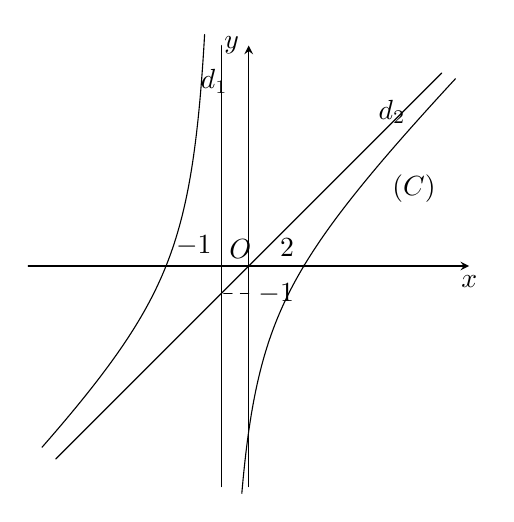
\begin{tikzpicture}[line join=round,line cap=round,>=stealth,scale=0.35]
		\draw[->] (-8,0)--(8,0) node[below] {$x$};
		\draw[->] (0,-8)--(0,8) node[left] {$y$};
		\draw (-1,-8)--(-1,8);
		\draw[dashed] (0,-1)--(-1,-1);
		\draw (-7,-7)--(7,7);
		\node at (-1.25,6.7) {$d_1$};
		\node at (5.2,5.6) {$d_2$};
		\node at (6,2.8) {$(C)$};
		\node[above] at (-0.3,-0.1) {$O$};
		\node[above left] at (-1,0) {$-1$};
		\node[right] at (0,-1) {$-1$};
		\node[above left] at (2,0) {$2$};
		\draw[smooth,samples=200,domain=-7.5:-1.6] plot(\x,{(\x)-6/(\x+1)});
		\draw[smooth,samples=200,domain=-0.25:7.5] plot(\x,{(\x)-6/(\x+1)});
		\coordinate (A) at (2,0);
		\foreach \p in {A} \fill (\p) circle (1.5pt);
	\end{tikzpicture}
	}
	\loigiai
	{
	\begin{itemchoice}
		\itemch Ta có $y(0)=\dfrac{-6}{1}=-6$.\\
		Vậy đồ thị không đi qua điểm $(0;2)$.
		\itemch Đồ thị có tiệm cận đứng là $x=-1$.
		\itemch Đồ thị có tiệm cận xiên là $y=x$.
		\itemch Hàm số có dạng $y=x+\dfrac{m}{x+1}$.
		Từ đồ thị, ta thấy đồ thị đi qua điểm $(2;0)$ nên $0=2+\dfrac{m}{3} \Leftrightarrow m=-6$.\\
		Vậy $ y=x-\dfrac{6}{x+1} =\dfrac{x^2+x-6}{x+1}$.\\
		Suy ra $a=1$, $b=1$, $c=-6$, $d=1$.\\
		$\Rightarrow a+b+c+d=1+1-6+1=-3<0$.
		\end{itemchoice}
	}
\end{ex}
\Closesolutionfile{ans}
\caukq
\Opensolutionfile{ans}[ans/ans-26-6-HaNoi-SoGD-L1-KQ]
\begin{ex}%[Đề thi thử Sở GD Hà Nội 2025-2026 L1]%[Thái Doãn Hùng, dự án đề THPT 2025 2026]%[1H8V6-2]
	\immini
	{Cho hình chóp tứ giác $S.ABCD$ có đáy $ABCD$ là hình vuông cạnh bằng $2$. Biết rằng $SA$ vuông góc với mặt phẳng $(ABCD)$ và $SA=\sqrt{6}$ \textit{(tham khảo hình vẽ)}. Góc phẳng nhị diện $[S,BD,C]$ có số đo bằng bao nhiêu độ?
	}
	{
	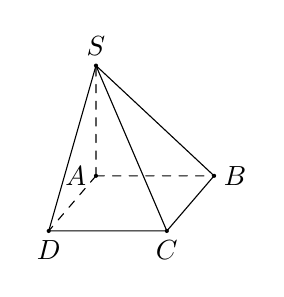
\begin{tikzpicture}[line join=round,line cap=round,>=stealth,scale=0.5]
		\coordinate (D) at (0,0);
		\coordinate (C) at (3,0);
		\coordinate (B) at (4.2,1.4);
		\coordinate (A) at (1.2,1.4);
		\coordinate (S) at (1.2,4.2);
		\draw (D) -- (C) (C) -- (B) (B) -- (S) (S) -- (D) (S) -- (C);
		\draw[dashed] (A) -- (B) (A) -- (D) (A) -- (S);
		\foreach \p in {S,A,B,C,D} \fill (\p) circle (1.5pt);
		\foreach \p in {D,C} \node[below] at (\p) {$\p$};
		\foreach \p in {B} \node[right] at (\p) {$\p$};
		\foreach \p in {A} \node[left] at (\p) {$\p$};
		\foreach \p in {S} \node[above] at (\p) {$\p$};
	\end{tikzpicture}
	}
	%\shortans{$120$}
	\loigiai
	{
	Gọi $O$ là giao điểm của hai đường chéo $AC$ và $BD$ của hình vuông $ABCD$.\\
	Vì $ABCD$ là hình vuông cạnh bằng $2$ nên $BD=2\sqrt{2}$.\\
	Suy $OB=\dfrac{BD}{2}=\sqrt{2}$.\\
	Ta có $ SA\perp (ABCD)$ nên $SA\perp BD$.\\
	Lại có $ AO\perp BD$.\\
	Suy ra mặt phẳng $(SAO)$ vuông góc với $BD$.\\
	Góc phẳng nhị diện $[S,BD,C]$ là góc giữa hai đường thẳng: $OS\subset (SBD), OC\subset (CBD)$.\\
	Vậy góc phẳng nhị diện cần tìm là $\widehat{SOC}$.\\
	Ta có $AO=\dfrac{AC}{2}=\sqrt{2}$.\\
	Xét tam giác vuông $SAO$: $SO=\sqrt{SA^2+AO^2}	=\sqrt{6+2}	=2\sqrt{2}$.\\
	Trong tam giác $SOC$: $ OS=2\sqrt{2}$ , $OC=\sqrt{2}$ , $SC=\sqrt{SA^2+AC^2}=\sqrt{6+8}=\sqrt{14}$.\\
	Áp dụng định lý cô-sin: $\cos\widehat{SOC}	=\dfrac{OS^2+OC^2-SC^2}{2\cdot OS\cdot OC}=\dfrac{8+2-14}{2\cdot 2\sqrt{2}\cdot \sqrt{2}} =-\dfrac{1}{2}$.\\
	Suy ra $\widehat{SOC}=120^\circ$.\\
	Vậy số đo góc phẳng nhị diện cần tìm bằng $120^\circ$.
	}
\end{ex}

\begin{ex}%[Đề thi thử Sở GD Hà Nội 2025-2026 L1]%[Thái Doãn Hùng, dự án đề THPT 2025 2026]%[1D6V3-5]
	Sau khi một loại thuốc kháng sinh được tiêm vào cơ thể thì nồng độ của thuốc trong máu sẽ giảm dần theo thời gian do quá trình chuyển hóa. Nồng độ thuốc trong máu sau $t$ giờ kể từ khi tiêm được mô hình hóa bởi công thức $C(t)=C_0\mathrm{e}^{-rt}\quad (\text{mg/lít})$. Trong đó:
	\begin{itemize}
	\item $C_0$ là nồng độ thuốc trong máu ngay sau khi tiêm.
	\item $r$ là hằng số dương đo tốc độ phân hủy của thuốc.
	\item $\mathrm{e}\approx 2{,}718$.
	\end{itemize}
	Biết rằng ngay sau khi tiêm, nồng độ thuốc trong máu là $15$ mg/lít và sau đó $4$ giờ nồng độ thuốc giảm còn $10$ mg/lít. Để đạt hiệu quả điều trị, bác sĩ sẽ tiêm lại một liều mới khi nồng độ thuốc trong máu của bệnh nhân giảm xuống và còn ít nhất $6$ mg/lít.\\
	Theo mô hình trên, để đạt hiệu quả điều trị thì khoảng thời gian nhiều nhất giữa hai lần tiêm thuốc là bao nhiêu giờ? \textit{(kết quả làm tròn đến hàng đơn vị)}
	%\shortans{$9$}
	\loigiai
	{
	Theo đề bài: $C(t)=15\mathrm{e}^{-rt}$.\\
	Sau $4$ giờ, nồng độ thuốc còn $10$ mg/lít nên $15\mathrm{e}^{-4r}=10$.\\
	Suy ra $\mathrm{e}^{-4r}=\dfrac{2}{3}$.\\
	Lấy lôgarit hai vế: $-4r=\ln\dfrac{2}{3}$ 
	nên $r=\dfrac{\ln \left( \dfrac{2}{3}\right)}{-4}$.\\
	Gọi $t$ là khoảng thời gian lớn nhất giữa hai lần tiêm thuốc. \\
	Khi đó: $C(t)=6$.\\
	Ta có $15\mathrm{e}^{-rt}=6 \Rightarrow \mathrm{e}^{-rt}=\dfrac{2}{5} \Rightarrow -rt=\ln\dfrac{2}{5}$.\\
	Suy ra $t=\dfrac{\ln\left( \dfrac{5}{2}\right)}{r}=	\dfrac{4\ln\left( \dfrac{5}{2}\right)}{\ln\left( \dfrac{3}{2}\right)} \approx 9{,}04$.\\
	Vậy khoảng thời gian nhiều nhất giữa hai lần tiêm thuốc là khoảng $9\text{giờ}$.
	}
\end{ex}

\begin{ex}%[Đề thi thử Sở GD Hà Nội 2025-2026 L1]%[Thái Doãn Hùng, dự án đề THPT 2025 2026]%[2D4C3-1]
	\immini{
	Trong lưới ô vuông có hai đường parabol như hình vẽ. Biết rằng mỗi ô vuông nhỏ có cạnh bằng $1$ cm. Diện tích của hình phẳng trong lưới ô vuông được giới hạn bởi hai đường parabol (phần gạch chéo) bằng bao nhiêu centimét vuông? \textit{(kết quả làm tròn đến hàng phần trăm)}
	}{
		\begin{tikzpicture}[line join=round,line cap=round,>=stealth,scale=0.6]
			\draw[gray!60] (0,0) grid (8,8);
			\draw[thick] (0,0) rectangle (8,8);
			\draw[smooth,samples=200,domain=0:8] plot(\x,{0.5*(\x-4)^2});
			\draw[purple,smooth,samples=200,domain=0:8] plot(\x,{11/48*\x*\x -47/24*\x +6});
			\begin{scope}
				\clip plot[smooth,samples=200,domain=0:8] (\x,{0.5*(\x-4)^2})--plot[smooth,samples=200,domain=8:0](\x,{11/48*\x*\x -47/24*\x +6})-- cycle;
				\fill[pattern=north east lines]	(0,0) rectangle (8,8);
			\end{scope}
			\coordinate (A) at (0,6);
			\coordinate (B) at (8,5);
			\coordinate (C) at (4,0);
			\coordinate (D) at (2,3);
			\foreach \p in {A,B,C,D} \fill (\p) circle (1.5pt);
		\end{tikzpicture}
	}
	%\shortans{$9{,}76$}
	\loigiai
	{
	Gắn hệ trục như hình vẽ, một đơn vị tương ứng với một ô
	\begin{center}
		\begin{tikzpicture}[line join=round,line cap=round,>=stealth,scale=0.6]
		\draw[gray!60] (0,0) grid (8,8);
		\draw[thick] (0,0) rectangle (8,8);
		\draw[->] (0,0)--(9,0) node[below] {$x$};
		\draw[->] (0,0)--(0,9) node[left] {$y$};
		\draw[smooth,samples=200,domain=0:8] plot(\x,{0.5*(\x-4)^2});
		\draw[purple,smooth,samples=200,domain=0:8] plot(\x,{11/48*\x*\x -47/24*\x +6});
		\begin{scope}
			\clip plot[smooth,samples=200,domain=0:8] (\x,{0.5*(\x-4)^2})--plot[smooth,samples=200,domain=8:0](\x,{11/48*\x*\x -47/24*\x +6})-- cycle;
			\fill[pattern=north east lines]	(0,0) rectangle (8,8);
		\end{scope}
		\coordinate (A) at (0,6);
		\coordinate (B) at (8,5);
		\coordinate (C) at (4,0);
		\coordinate (D) at (2,3);
		\foreach \p in {A,B,C,D} \fill (\p) circle (1.5pt);
		\node[below] at (4,0) {$4$};
		\node[below] at (8,0) {$8$};
		\node[left] at (0,0) {$0$};
		\node[left] at (0,8) {$8$};
		\node[left] at (0,6) {$6$};
		\end{tikzpicture}
	\end{center}
	Từ hình vẽ, ta xác định được:
	\begin{itemize}
		\item Parabol phía dưới có đỉnh $(4;0)$ và đi qua điểm $(0;8)$ nên có phương trình $y=\dfrac{1}{2}(x-4)^2$.
		\item Parabol phía trên đi qua ba điểm $(0;6)$, $(2;3)$ , $(8;5)$ nên có phương trình $y=\dfrac{11}{48}x^2-\dfrac{47}{24}x+6$.
	\end{itemize}
	Diện tích hình phẳng cần tìm là 
	\begin{align*}
		S& =\displaystyle \int\limits_0^8 \left|\dfrac12(x-4)^2-\left(\dfrac{11}{48}x^2-\dfrac{47}{24}x+6\right)\right|\mathrm{\,d}x.\\
		&=\int\limits_0^8\left|\dfrac{13}{48}x^2-\dfrac{49}{24}x+2\right|\mathrm{\,d}x\approx 9{,}76.
	\end{align*}
	Vậy diện tích hình phẳng cần tìm xấp xỉ $9{,}76\text{ cm}^2$.
	}
\end{ex}

\begin{ex}%[Đề thi thử Sở GD Hà Nội 2025-2026 L1]%[Thái Doãn Hùng, dự án đề THPT 2025 2026]%[0D8C1-4]
	\immini{
	Người ta trang trí một bảng ô vuông $4\times 4$ (như hình $1$) bởi các ngôi sao và các bông hoa giống nhau. Mỗi ô vuông nhỏ được dán một ngôi sao hoặc một bông hoa, sao cho trong mỗi hàng hoặc mỗi cột của bảng ô vuông đều có $2$ ngôi sao và $2$ bông hoa (tham khảo một cách dán trong hình $2$). Có tất cả bao nhiêu cách trang trí bảng ô vuông thỏa mãn yêu cầu trên?
	}{
		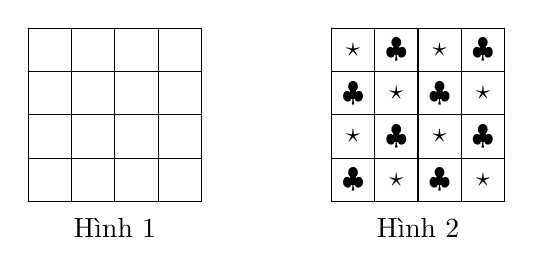
\begin{tikzpicture}[line join=round,line cap=round,>=stealth,scale=0.55]
			\foreach \x in {0,1,2,3,4}{\draw (\x,0)--(\x,4);\draw (0,\x)--(4,\x);}
			\node at (2,-0.6) {Hình 1};
			\begin{scope}[xshift=7cm]
				\foreach \x in {0,1,2,3,4}{\draw (\x,0)--(\x,4);\draw (0,\x)--(4,\x);}
				\foreach \i in {0,1,2,3}{\foreach \j in {0,1,2,3} {\pgfmathtruncatemacro{\k}{mod(\i+\j,2)}\ifnum\k=0\node at (\i+0.5,3.5-\j) {$\star$};\else \node at (\i+0.5,3.5-\j) {$\clubsuit$};\fi}}
				\node at (2,-0.6) {Hình 2};
			\end{scope}
		\end{tikzpicture}
	}
	%\shortans{$2502$}
	\loigiai
	{
	Gọi:
	\begin{itemize}
	\item $A$ là biến cố: “Mỗi hàng của bảng đều có đúng $2$ ngôi sao”.
	\item $B$ là biến cố: “Mỗi cột của bảng đều có đúng $2$ ngôi sao”.	
	\end{itemize}
	Mỗi hàng của bảng gồm $4$ ô và cần chọn đúng $2$ ô để dán ngôi sao.\\
	Số cách chọn cho một hàng là $\mathrm{C}_4^2=6$.\\
	Vì bảng có $4$ hàng nên số cách thỏa mãn biến cố $A$ là $n(A)=6^4=1\,296$.\\
	Tương tự, số cách thỏa mãn biến cố $B$ là $n(B)=6^4=1\,296$.\\
	Ta có $A\cap B$ là biến cố: 
	"Mỗi hàng và mỗi cột đều có đúng $2$ ngôi sao".\\
	Để tính số phần tử của $A\cap B$, ta đếm số bảng $4\times4$ sao cho: mỗi hàng và mỗi cột đều có đúng $2$ ngôi sao.\\
	Mỗi hàng tương ứng với một cách chọn $2$ vị trí trong $4$ vị trí.\\
	Coi ngôi sao là số $1$ và bông hoa là số $0$. Các kiểu hàng có thể có là: \\
	$1\,1\,0\,0$; \quad $1\,0\,1\,0$;\quad $1\,0\,0\,1$; \quad $0\,1\,1\,0$;\quad $0\,1\,0\,1$; \quad$0\,0\,1\,1$.\\
	Có tất cả $\mathrm{C}_4^2=6$ kiểu hàng.\\
	Ta lập bảng gồm $4$ hàng từ các kiểu trên sao cho trong mỗi cột cũng xuất hiện đúng hai số $1$.\\
	Sau khi xét tất cả các khả năng thỏa mãn đồng thời:
	\begin{itemize}
	\item mỗi hàng có đúng $2$ số $1$;
	\item mỗi cột có đúng $2$ số $1$;
	\end{itemize}
	ta thu được tất cả $90$ bảng thỏa mãn.\\
	Vì vậy: $ n(A\cap B)=90$.\\
	Theo công thức cộng: $n(A\cup B) =n(A)+n(B)-n(A\cap B)$.\\
	Suy ra $n(A\cup B) =1\, 296+1\,296-90=2\,502$.\\
	Vậy có tất cả $ 2\,502$ cách trang trí bảng ô vuông.
	}
\end{ex}

\begin{ex}%[Đề thi thử Sở GD Hà Nội 2025-2026 L1]%[Thái Doãn Hùng, dự án đề THPT 2025 2026]%[1D2V2-7]
	Anh Tú vay ngân hàng $300$ triệu đồng để mua xe ô tô với lãi suất cố định $7{,}2\%$/năm theo hình thức trả góp hằng tháng, trong thời hạn $12$ tháng (ứng với $12$ kì trả nợ). Trong thời hạn đó, cuối mỗi kì trả nợ, anh Tú phải trả $25$ triệu đồng tiền gốc (ứng với $300$ triệu đồng chia đều cho $12$ tháng) và một khoản tiền lãi được tính theo số tiền dư nợ còn lại. Sau $12$ tháng, tổng số tiền lãi anh Tú phải trả ngân hàng là bao nhiêu triệu đồng? \textit{(kết quả làm tròn đến hàng phần mười)}
	%\shortans{$11{,}7$}
	\loigiai
	{
	Lãi suất theo tháng là $\dfrac{7{,}2\%}{12}=0{,}6\%=0{,}006$.\\
	Mỗi tháng anh Tú trả $\dfrac{300}{12}=25$ triệu đồng tiền gốc.\\
	Số dư nợ đầu mỗi tháng lần lượt là $300$; $275$; $250$; $\ldots$; $25$.\\
	Đây là một cấp số cộng với: $u_1=300$, $u_{12}=25$, $n=12$.\\
	Tổng số dư nợ dùng để tính lãi là $S=\dfrac{12(300+25)}{2}=1\,950$.\\
	Tổng số tiền lãi phải trả là $0{,}006\cdot 1950=11{,}7$ (triệu đồng).\\
	Vậy sau $12$ tháng, tổng số tiền lãi anh Tú phải trả là $11{,}7$ triệu đồng.
	}
\end{ex}

\begin{ex}%[Đề thi thử Sở GD Hà Nội 2025-2026 L1]%[Thái Doãn Hùng, dự án đề THPT 2025 2026]%[2D1C3-6]
	\immini
	{Cho hình vuông $ABCD$ có độ dài cạnh bằng $1$. Cung $AC$ là một phần tư đường tròn tâm $D$, bán kính $DA$ (tham khảo hình vẽ). Giả sử $P$ là điểm thay đổi trên cung $AC$ ($P$ khác $A$ và $C$). Tiếp tuyến tại điểm $P$ của cung $AC$ cắt các đoạn thẳng $AB$, $BC$ theo thứ tự tại các điểm $M$, $N$. Diện tích lớn nhất của tam giác $BMN$ bằng bao nhiêu? \textit{(kết quả làm tròn đến hàng phần trăm)}
	}
	{
	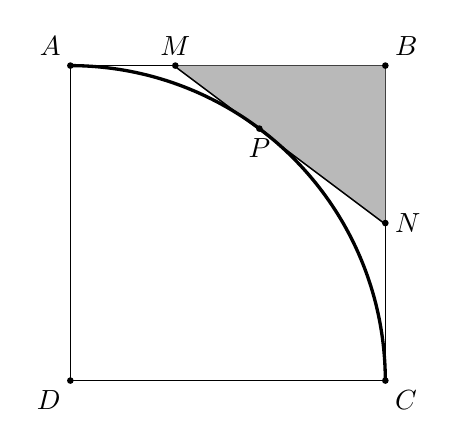
\begin{tikzpicture}[line join=round,line cap=round,>=stealth,scale=0.8]
		\coordinate (D) at (0,0);
		\coordinate (C) at (5,0);
		\coordinate (B) at (5,5);
		\coordinate (A) at (0,5);
		\coordinate (P) at ({3,4});
		\coordinate (M) at ({5/3,5});
		\coordinate (N) at ({5,2.5});
		\draw (A)--(B)--(C)--(D)--cycle;
		\draw[line width=1.2pt] (M)--(N);
		\fill[gray!55] (M)--(B)--(N)--cycle;
		\draw[black!100,very thick] plot[smooth,samples=200,domain=0:90] ({5*cos(\x)},{5*sin(\x)});
		\foreach \p in {A,B,C,D,P} \fill (\p) circle (1.5pt);
		\foreach \p in {M,N} \fill (\p) circle (1.5pt);
		\foreach \p in {A} \node[above left] at (\p) {$\p$};
		\foreach \p in {B} \node[above right] at (\p) {$\p$};
		\foreach \p in {C} \node[below right] at (\p) {$\p$};
		\foreach \p in {D} \node[below left] at (\p) {$\p$};
		\node[above] at (M) {$M$};
		\node[right] at (N) {$N$};
		\node[below] at (P) {$P$};
	\end{tikzpicture}
	}
	%\shortans{$0{,}17$}
	\loigiai
	{
	Đặt $AM=MP=x$ với $0<x<1$.\\
	Khi đó: $BM=1-x$.\\\
	Tương tự, đặt $PN=NC=y$.\\
	Suy ra $BN=1-y$.\\
	Vì tam giác $BMN$ vuông tại $B$ nên $S_{BMN}=\dfrac12(1-x)(1-y)$.\\
	Mặt khác: $MN=MP+PN=x+y$.\\
	Áp dụng định lí Py-ta-go trong tam giác vuông $BMN$: 
	\begin{align*}
		MN^2 =	BM^2+BN^2 &\Rightarrow (x+y)^2 = (1-x)^2+(1-y)^2.\\
		&\Leftrightarrow x^2+2xy+y^2 = 1-2x+x^2+1-2y+y^2.\\
		&\Leftrightarrow xy+x+y=1. \\
		&\Rightarrow y=\dfrac{1-x}{x+1}.\\
	\end{align*}
	Khi đó: $ S(x) = \dfrac12(1-x) \left(1-\dfrac{1-x}{x+1}\right)=\dfrac{x(1-x)}{x+1}$.\\
	Xét hàm số $f(x)=\dfrac{x(1-x)}{x+1}, \qquad 0<x<1$.\\
	Ta có $f'(x) =\dfrac{1-2x-x^2}{(x+1)^2}$.\\
	Giải phương trình $f'(x)=0 $ ta được $x=\sqrt2-1$.\\
	Ta có bảng biến thiên sau:
	\begin{center}
		
\begin{tikzpicture}
		\tkzTabInit[nocadre=false,lgt=1.2,espcl=3]
		{$x$/1,$y'$/1,$y$/2.5}
		{$0$,$\sqrt{2}-1$,$1$}		
		\tkzTabLine{,+,0,-,}
		\tkzTabVar{-/$0$,+/$3-2\sqrt{2}$,-/$0$}
		\end{tikzpicture}
	\end{center}
	Hàm số đạt giá trị lớn nhất tại $x=\sqrt2-1, S_{\max} = f(\sqrt2-1)	=3-2\sqrt2\approx 0{,}17$.\\
	Vậy diện tích lớn nhất của tam giác $BMN$ xấp xỉ $0{,}17$.
	}
\end{ex}

\Closesolutionfile{ans}

%\indapan{6}{ans/ans-26-6-HaNoi-SoGD-L1-LC}
%\indapan{4}{ans/ans-26-6-HaNoi-SoGD-L1-DS}
%\indapan{6}{ans/ans-26-6-HaNoi-SoGD-L1-KQ}